\documentclass[border=5pt]{standalone}
\usepackage[defaultfam,tabular,lining]{montserrat}
\usepackage[T1]{fontenc}
\renewcommand{\familydefault}{\sfdefault}
\usepackage[eulergreek]{sansmath}
\sansmath
\usepackage{tikz}
\usetikzlibrary{arrows.meta, positioning, calc}
\usepackage{fontawesome5}

% Palette (matching fl-comparison.tex / architecture.tex)
\definecolor{inkblack}{HTML}{111111}
\definecolor{pbpurple}{HTML}{6D28D9}
\definecolor{pbpurplefill}{HTML}{F5F3FF}
\definecolor{warnred}{HTML}{B91C1C}
\definecolor{warnredfill}{HTML}{FEF2F2}
\definecolor{devicegrey}{HTML}{94A3B8}
\definecolor{devicefill}{HTML}{E2E8F0}
\definecolor{trustteal}{HTML}{0D9488}
\definecolor{trusttealfill}{HTML}{F0FDFA}
\definecolor{dimgrey}{HTML}{C4B5FD}

\begin{document}
\begin{tikzpicture}[
    font=\footnotesize,
    dnode/.style={draw=inkblack, fill=white, rounded corners=3pt,
                  minimum height=0.7cm, minimum width=2.0cm, align=center,
                  line width=1.0pt, text=inkblack},
    lnode/.style={draw=inkblack, fill=white, rounded corners=3pt,
                  minimum height=0.6cm, minimum width=1.3cm, align=center,
                  line width=1.0pt, text=inkblack, font=\scriptsize},
    lnodeHL/.style={draw=pbpurple, fill=pbpurplefill, rounded corners=3pt,
                    minimum height=0.6cm, minimum width=1.3cm, align=center,
                    line width=1.2pt, text=inkblack, font=\scriptsize},
    lnodeWarn/.style={draw=warnred, fill=warnredfill, rounded corners=3pt,
                      minimum height=0.6cm, minimum width=1.3cm, align=center,
                      line width=1.2pt, text=inkblack, font=\scriptsize},
    bcell/.style={draw=inkblack, fill=white, minimum height=0.44cm,
                  minimum width=0.95cm, align=center, line width=0.8pt,
                  text=inkblack, font=\tiny, inner sep=0.5pt, outer sep=0pt},
    bcellHL/.style={bcell, draw=pbpurple, fill=pbpurplefill, line width=1.0pt},
    scell/.style={draw=inkblack, fill=white, minimum height=0.36cm,
                  minimum width=0.5cm, align=center, line width=0.6pt,
                  text=inkblack, font=\fontsize{4}{4.8}\selectfont,
                  inner sep=0.5pt, outer sep=0pt},
    binlbl/.style={font=\tiny, text=inkblack!60, inner sep=1pt},
    rowlbl/.style={font=\tiny, text=inkblack!60, inner sep=1pt, anchor=east},
    arr/.style={-{Stealth[length=5pt,width=3.5pt]}, line width=1.1pt, inkblack},
    arrwarn/.style={-{Stealth[length=5pt,width=3.5pt]}, line width=1.1pt, warnred},
    arrpb/.style={-{Stealth[length=5pt,width=3.5pt]}, line width=1.1pt, pbpurple},
    arrdim/.style={-{Stealth[length=5pt,width=3.5pt]}, line width=1.1pt, dimgrey, densely dashed},
    edge/.style={line width=1.0pt, inkblack},
    edgewarn/.style={line width=1.2pt, warnred},
    lbl/.style={font=\scriptsize\bfseries, text=inkblack, inner sep=2pt},
  ]

  % ===== PANEL (a): Without Path Hiding =====
  \begin{scope}

    \node[font=\normalsize\bfseries, text=inkblack] at (3.5, 6.5) {(a) Without Path Hiding (Node Tag Leaks)};

    % Root node
    \node[dnode] (rA) at (3.5, 5.5) {glucose $\leq$ 140};

    % Level 1
    \node[dnode] (l1A) at (1.5, 4.0) {age $\leq$ 50};
    \node[dnode] (r1A) at (5.5, 4.0) {bmi $\leq$ 30};

    % Leaves
    \node[lnode] (lA) at (-0.7, 2.5) {Leaf A};
    \node[lnodeWarn] (lB) at (2.3, 2.5) {Leaf B};
    \node[lnode] (lC) at (5.3, 2.5) {Leaf C};
    \node[lnode] (lD) at (7.8, 2.5) {Leaf D};

    % Tree edges — highlighted path in warnred
    \draw[edgewarn] (rA.south) -- (l1A.north);
    \draw[edge] (rA.south) -- (r1A.north);
    \draw[edge] (l1A.south) -- (lA.north);
    \draw[edgewarn] (l1A.south) -- (lB.north);
    \draw[edge] (r1A.south) -- (lC.north);
    \draw[edge] (r1A.south) -- (lD.north);

    % Bin grid under Leaf B only, with range annotations
    % Row 1: glucose (4 bins), labels above
    \node[binlbl] at (0.875, 1.98) {$\leq$100};
    \node[binlbl] at (1.825, 1.98) {100--140};
    \node[binlbl] at (2.775, 1.98) {140--180};
    \node[binlbl] at (3.725, 1.98) {$>$180};
    \node[rowlbl] at (0.3, 1.64) {glucose};
    \node[bcell]   (aG1) at (0.875, 1.64) {(0,0)};
    \node[bcellHL] (aG2) at (1.825, 1.64) {(g,h)};
    \node[bcell]   (aG3) at (2.775, 1.64) {(0,0)};
    \node[bcell]   (aG4) at (3.725, 1.64) {(0,0)};
    % More features between the two shown rows
    \fill[inkblack!75] (2.3, 1.08) circle (1.0pt);
    \fill[inkblack!75] (2.3, 1.22) circle (1.0pt);
    \fill[inkblack!75] (2.3, 1.36) circle (1.0pt);
    % Row 2: smoking (3 bins), labels below
    \node[rowlbl] at (0.3, 0.80) {smoking};
    \node[bcell]   (aS1) at (1.35, 0.80) {(0,0)};
    \node[bcell]   (aS2) at (2.30, 0.80) {(0,0)};
    \node[bcellHL] (aS3) at (3.25, 0.80) {(g,h)};

    % Client
    \node[font=\scriptsize, text=pbpurple] (cliA) at (2.3, -0.25) {{\normalsize\faUser}};
    \node[font=\scriptsize\bfseries, text=pbpurple] at (2.3, -0.65) {Client $i$};
    \node[font=\tiny, text=inkblack!60] at (2.3, -1.0) {glucose 121 $\cdot$ smoking current};

    % Arrow: client -> Leaf B grid (ends below the category labels, head visible)
    \draw[arrwarn] (cliA.north) -- (2.3, 0.34);
    \node[binlbl, fill=white] at (1.35, 0.46) {never};
    \node[binlbl, fill=white] at (2.30, 0.46) {former};
    \node[binlbl, fill=white] at (3.25, 0.46) {current};
    \node[font=\scriptsize\bfseries, text=inkblack, anchor=east] at (1.6, 0.12) {shares};

    % Caption box
    \node[fill=warnredfill, rounded corners=4pt, inner sep=8pt, text width=8.4cm, align=center]
      at (3.5, -2.1) {
        {\bfseries\textcolor{warnred}{Node tag reveals the client's tree path}}\\[3pt]
        {\scriptsize but not the bin: every submission covers all bins of all features}
      };

  \end{scope}

  % ===== PANEL (b): With Path Hiding =====
  \begin{scope}[xshift=11.8cm]

    \node[font=\normalsize\bfseries, text=inkblack] at (3.5, 6.5) {(b) With Path Hiding (Indistinguishability)};

    % Root node
    \node[dnode] (rB) at (3.5, 5.5) {glucose $\leq$ 140};

    % Level 1
    \node[dnode] (l1B) at (1.5, 4.0) {age $\leq$ 50};
    \node[dnode] (r1B) at (5.5, 4.0) {bmi $\leq$ 30};

    % Leaves — all with pbpurple tint
    \node[lnodeHL] (lAb) at (-0.7, 2.5) {Leaf A};
    \node[lnodeHL] (lBb) at (2.3, 2.5) {Leaf B};
    \node[lnodeHL] (lCb) at (5.3, 2.5) {Leaf C};
    \node[lnodeHL] (lDb) at (7.8, 2.5) {Leaf D};

    % Tree edges — all same color (no path visible)
    \draw[edge] (rB.south) -- (l1B.north);
    \draw[edge] (rB.south) -- (r1B.north);
    \draw[edge] (l1B.south) -- (lAb.north);
    \draw[edge] (l1B.south) -- (lBb.north);
    \draw[edge] (r1B.south) -- (lCb.north);
    \draw[edge] (r1B.south) -- (lDb.north);

    % True-node grid under Leaf B: enlarged, with range annotations
    \node[binlbl] at (0.875, 1.98) {$\leq$100};
    \node[binlbl] at (1.825, 1.98) {100--140};
    \node[binlbl] at (2.775, 1.98) {140--180};
    \node[binlbl] at (3.725, 1.98) {$>$180};
    \node[bcell]   (bBG1) at (0.875, 1.64) {(0,0)};
    \node[bcellHL] (bBG2) at (1.825, 1.64) {(g,h)};
    \node[bcell]   (bBG3) at (2.775, 1.64) {(0,0)};
    \node[bcell]   (bBG4) at (3.725, 1.64) {(0,0)};
    \fill[inkblack!75] (2.3, 1.08) circle (1.0pt);
    \fill[inkblack!75] (2.3, 1.22) circle (1.0pt);
    \fill[inkblack!75] (2.3, 1.36) circle (1.0pt);
    \node[bcell]   (bBS1) at (1.35, 0.80) {(0,0)};
    \node[bcell]   (bBS2) at (2.30, 0.80) {(0,0)};
    \node[bcellHL] (bBS3) at (3.25, 0.80) {(g,h)};

    % Decoy grids under Leaves A, C, D: smaller, all-zero
    \node[rowlbl] at (-1.8, 1.64) {glucose};
    \node[rowlbl] at (-1.8, 0.96) {smoking};
    % Leaf A
    \node[scell] (bAG1) at (-1.45, 1.64) {(0,0)};
    \node[scell] (bAG2) at (-0.95, 1.64) {(0,0)};
    \node[scell] (bAG3) at (-0.45, 1.64) {(0,0)};
    \node[scell] (bAG4) at ( 0.05, 1.64) {(0,0)};
    \fill[inkblack!75] (-0.7, 1.20) circle (0.8pt);
    \fill[inkblack!75] (-0.7, 1.30) circle (0.8pt);
    \fill[inkblack!75] (-0.7, 1.40) circle (0.8pt);
    \node[scell] (bAS1) at (-1.20, 0.96) {(0,0)};
    \node[scell] (bAS2) at (-0.70, 0.96) {(0,0)};
    \node[scell] (bAS3) at (-0.20, 0.96) {(0,0)};
    % Leaf C
    \node[scell] (bCG1) at (4.55, 1.64) {(0,0)};
    \node[scell] (bCG2) at (5.05, 1.64) {(0,0)};
    \node[scell] (bCG3) at (5.55, 1.64) {(0,0)};
    \node[scell] (bCG4) at (6.05, 1.64) {(0,0)};
    \fill[inkblack!75] (5.3, 1.20) circle (0.8pt);
    \fill[inkblack!75] (5.3, 1.30) circle (0.8pt);
    \fill[inkblack!75] (5.3, 1.40) circle (0.8pt);
    \node[scell] (bCS1) at (4.80, 0.96) {(0,0)};
    \node[scell] (bCS2) at (5.30, 0.96) {(0,0)};
    \node[scell] (bCS3) at (5.80, 0.96) {(0,0)};
    % Leaf D
    \node[scell] (bDG1) at (7.05, 1.64) {(0,0)};
    \node[scell] (bDG2) at (7.55, 1.64) {(0,0)};
    \node[scell] (bDG3) at (8.05, 1.64) {(0,0)};
    \node[scell] (bDG4) at (8.55, 1.64) {(0,0)};
    \fill[inkblack!75] (7.8, 1.20) circle (0.8pt);
    \fill[inkblack!75] (7.8, 1.30) circle (0.8pt);
    \fill[inkblack!75] (7.8, 1.40) circle (0.8pt);
    \node[scell] (bDS1) at (7.30, 0.96) {(0,0)};
    \node[scell] (bDS2) at (7.80, 0.96) {(0,0)};
    \node[scell] (bDS3) at (8.30, 0.96) {(0,0)};

    % Client
    \node[font=\scriptsize, text=pbpurple] (cliB) at (2.3, -0.25) {{\normalsize\faUser}};
    \node[font=\scriptsize\bfseries, text=pbpurple] at (2.3, -0.65) {Client $i$};
    \node[font=\tiny, text=inkblack!60] at (2.3, -1.0) {glucose 121 $\cdot$ smoking current};

    % Arrows (drawn before the smoking labels; labels overlay with white fill)
    \draw[arrpb] (cliB.north) -- (2.3, 0.34);
    \draw[arrdim] (cliB.north) -- (bAS2.south);
    \draw[arrdim] (cliB.north) -- (bCS2.south);
    \draw[arrdim] (cliB.north) -- (bDS2.south);
    \node[binlbl, fill=white] at (1.35, 0.46) {never};
    \node[binlbl, fill=white] at (2.30, 0.46) {former};
    \node[binlbl, fill=white] at (3.25, 0.46) {current};
    \node[font=\scriptsize\bfseries, text=inkblack, anchor=east] at (0.2, 0.2) {shares};

    % Caption box
    \node[fill=trusttealfill, rounded corners=4pt, inner sep=8pt, text width=8.5cm, align=center]
      at (3.5, -2.1) {
        {\bfseries\textcolor{trustteal}{Neither leaf nor bin is distinguishable}}\\[3pt]
        {\scriptsize Decoy leaves receive all-zero vectors; shares of $0$ look identical to real shares}
      };

  \end{scope}

\end{tikzpicture}
\end{document}
